%%%%%%%%%%%%%%%%%%%%%%%%%%%%%%%%%%%%%%%%%
% Beamer Presentation
% LaTeX Template
% Version 1.0 (10/11/12)
%
% This template has been downloaded from:
% http://www.LaTeXTemplates.com
%
% License:
% CC BY-NC-SA 3.0 (http://creativecommons.org/licenses/by-nc-sa/3.0/)
%
%%%%%%%%%%%%%%%%%%%%%%%%%%%%%%%%%%%%%%%%%

%----------------------------------------------------------------------------------------
%	PACKAGES AND THEMES
%----------------------------------------------------------------------------------------

\documentclass{beamer}
\mode<presentation> {
\usetheme{PaloAlto}}
\usepackage{graphicx} % Allows including images
\usepackage{booktabs} % Allows the use of \toprule, \midrule and \bottomrule in tables
\usepackage{color, colortbl}
\graphicspath{{images/}}


%----------------------------------------------------------------------------------------
%	TITLE PAGE
%----------------------------------------------------------------------------------------

\logo{
\includegraphics[scale=0.05]{sim}}
%\definecolor{TeamSim}{RGB}{15,37,51}
\definecolor{TeamSim}{RGB}{6,54,142}
\setbeamercolor{structure}{fg=TeamSim}

\title[Welcome]{7CCSMGPR - Traffic Simulation Project} % The short title appears at the bottom of every slide, the full title is only on the title page

\author{\textbf{Team Simulus}} % Your name
\institute[KCL] % Your institution as it will appear on the bottom of every slide, may be shorthand to save space
{
King's College London \\ % Your institution for the title page
\medskip
\textit{https://github.com/leorohr/simulus} % Your email address
}
\date{11 February 2015} % Date, can be changed to a custom date

\begin{document}

\begin{frame}
\titlepage % Print the title page as the first slide
\end{frame}


%----------------------------------------------------------------------------------------
%	PRESENTATION SLIDES
%----------------------------------------------------------------------------------------

%------------------------------------------------
\section{Project Description} % Sections can be created in order to organize your presentation into discrete blocks, all sections and subsections are automatically printed in the table of contents as an overview of the talk
%------------------------------------------------

\subsection{Aims} % A subsection can be created just before a set of slides with a common theme to further break down your presentation into chunks

\begin{frame}
\frametitle{Aims (through MoSCoW Analysis)}

\begin{itemize}
\item \textbf{Must}
	\begin{itemize}
		\item Individual Vehicles
		\item Vehicle Entrance and Exit 
		\item Vehicle Behaviour
		\item Statistics - Delay, Average Speed, Distance Travelled
		\item Traffic Management Policies - traffic signal timing, speed limit, etc
	\end{itemize}
\item \textbf{Should}
	\begin{itemize}
		\item Emergency Services
		\item User Maps (Map Editor)
	\end{itemize}
\item \textbf{Could}
	\begin{itemize}
		\item Save/Load User Maps
		\item External Map Source e.g. Google Maps
		\end{itemize}
\item \textbf{Won't}
	\begin{itemize}
		\item Pre-existing Traffic Simulators or Libraries
	\end{itemize}	
\end{itemize}

\end{frame}

%------------------------------------------------
\section{Project Organisation}
%------------------------------------------------

\begin{frame}
\frametitle{Project Organisation}

\begin{itemize}
\item \textbf{Working Policy}
	\begin{itemize}
		\item Cooperation
		\item Equality
		\item Responsibility
		\item Self-Organisation
	\end{itemize}
\item \textbf{Methodology}
	\begin{itemize}
		\item Constraint - Time Pressure
		\item Iterative and Incremental
		\item Emphasis on Feedback
	\end{itemize}
\item \textbf{Flexible Roles}
	\begin{itemize}
		\item Research and Designer
		\item Developer – GUI, Model Implementation
		\item Documentation Analyst
	\end{itemize}
\item \textbf{Collaboration}
	\begin{itemize}
		\item Meetings, GitHub, Facebook, WhatsApp
	\end{itemize}	
\item \textbf{Peer Assessment and Conflict Resolution}
	\begin{itemize}
		\item Equal Weighting
		\item Voice, Vote, Resolve
	\end{itemize}	
\end{itemize}

\end{frame}

%------------------------------------------------
\section{Progress}
%------------------------------------------------

\begin{frame}
\frametitle{Progress}
%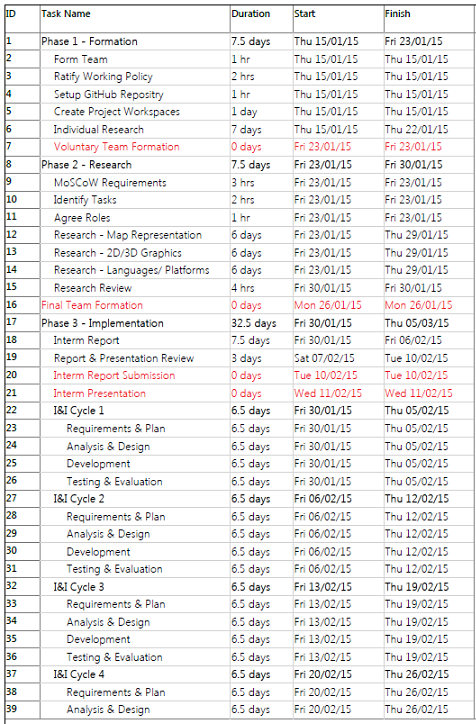
\includegraphics[scale=0.35]{gantt01}
%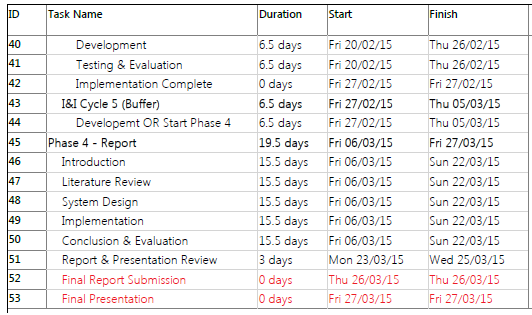
\includegraphics[scale=0.35]{gantt02}

\definecolor{LightCyan}{rgb}{0.88,1,1}

	\begin{tabular}{|c|l|}
	\hline
	\textbf{Date} & \textbf{Phase} \\ \hline
	15/01/15 & Formation \& Research \\ \hline
	23/01/15 & Research \\ \hline
	30/01/15 & Development Cycle 1 \\ \hline
	\rowcolor{LightCyan}
	06/02/15 & Development Cycle 2 \\ \hline
	13/02/15 & Development Cycle 3 \\ \hline
	20/02/15 & Development Cycle 4 \\ \hline
	27/02/15 & \textbf{Buffer (Development or Report)} \\ \hline
	06/03/15 & Report \\ \hline
	27/03/15 & Submission \\ \hline
	\end{tabular}
	
\end{frame}

%------------------------------------------------
\section{Demonstration}
%------------------------------------------------

\begin{frame}
\frametitle{Demonstration}
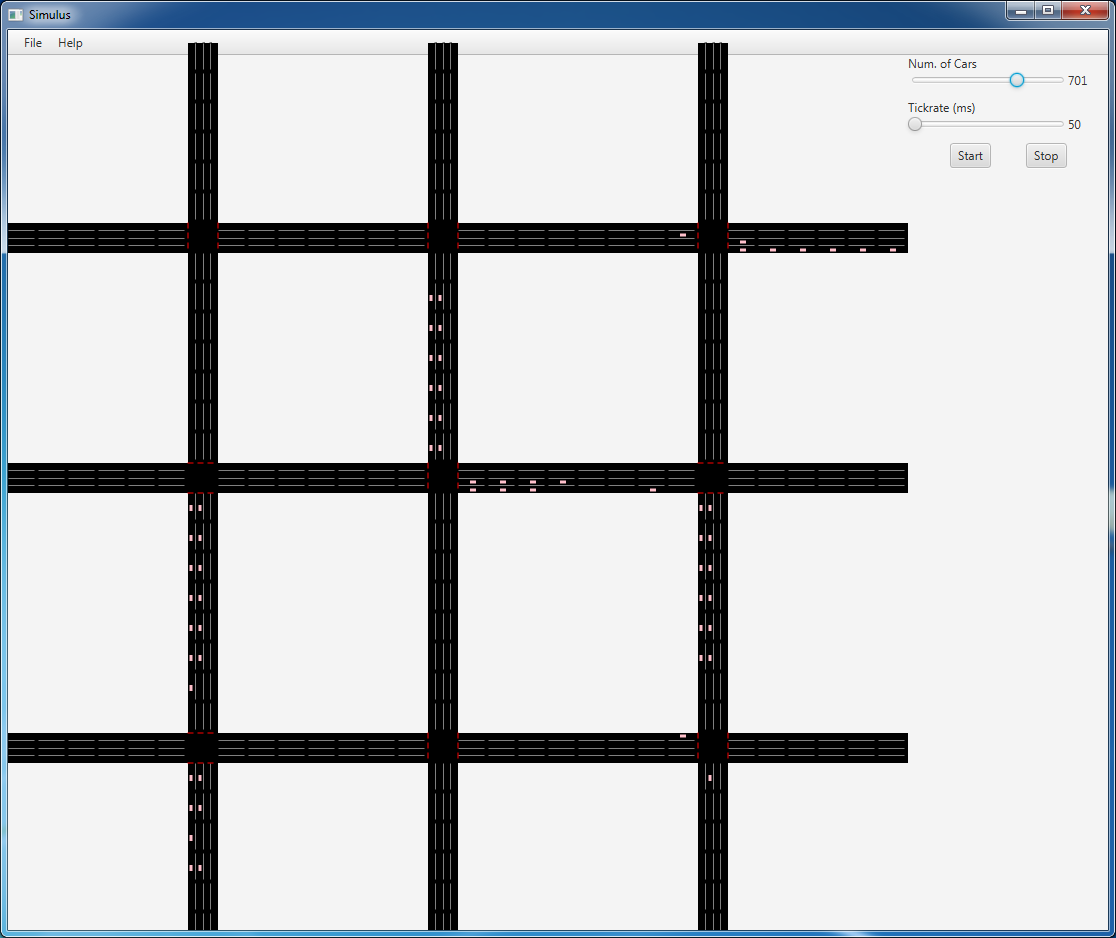
\includegraphics[scale=0.28]{screenshot}
\end{frame}

%------------------------------------------------
\section{Questions}
%------------------------------------------------

\begin{frame}
\frametitle{Questions}

\end{frame}

\end{document}